% Source of the template:
% https://fit.cvut.cz/cs/studium/programy-a-obory/doktorske/dsp-informatika/pro-stavajici-studenty/sablony
% Šablona prezentace

% Original presentation:
% https://github.com/filipbartek/neural-precedence-recommender/blob/master/presentation.tex

%\documentclass[a4paper,notes]{beamer}
\documentclass[a4paper]{beamer}

\setbeamertemplate{footline}[page number]
%
% Josef Hlavac & Tomas Zahradnicky (21.10.2010)
%
%\usepackage{pgfpages}
%\pgfpagesuselayout{4 on 1}[a4paper,border shrink=5mm,landscape]
%\pgfpagesuselayout{resize}[a4paper,border shrink=5mm,landscape]
\usepackage[utf8]{inputenc}
\usepackage{color}
\usetheme{Frankfurt}
\useinnertheme{circles}
\usepackage{subfigure}
\usepackage[english]{babel}

% glossaries should be loaded after hyperref.
\usepackage{glossaries}

% https://tex.stackexchange.com/q/25805/202639
\glsdisablehyper

\newacronym{ai}{AI}{artificial intelligence}
\newacronym{ann}{ANN}{artificial \acrlong{nn}}
\newacronym{atp}{ATP}{automated theorem prover}

\newacronym{cade}{CADE}{Conference on Automated Deduction}
% https://www.cadeinc.org/

\newacronym{cade-28}{CADE-28}{The 28th International \acrlong*{cade}}
% https://www.cs.cmu.edu/~mheule/CADE28/

\newacronym{casc}{CASC}{\Acrshort*{cade} \acrshort*{atp} System Competition}
% http://www.tptp.org/CASC/

\newacronym{ciirc}{CIIRC}{Czech Institute of Informatics, Robotics and Cybernetics}
\newacronym{cnf}{CNF}{clause normal form}
\newacronym{csv}{CSV}{comma-separated values}
\newacronym{ctu}{CTU}{Czech Technical University in Prague}
\newacronym{cv}{CV}{computer vision}
\newacronym{dag}{dag}{directed acyclic graph}
\newacronym{fel}{FEL}{Faculty of Electrical Engineering}
\newacronym{fof}{FOF}{first-order form}
% http://www.tptp.org/TPTP/TR/TPTPTR.shtml
\newacronym{fol}{FOL}{first-or\-der logic}
\newacronym{gcn}{GCN}{graph convolutional network}
\newacronym{gnn}{GNN}{graph \acrlong{nn}}
\newacronym{hin}{HIN}{heterogeneous information network}
\newacronym{json}{JSON}{JavaScript Object Notation}
\newacronym{kbo}{KBO}{Knuth-Bendix ordering}
\newacronym{lpo}{LPO}{lexicographic path ordering}
%\newacronym{ml}{ML}{machine learning}
\newacronym{nlp}{NLP}{natural language processing}
\newacronym{nn}{NN}{neural network}

\newacronym{paar}{PAAR}{Workshop on Practical Aspects of Automated Reasoning}
% http://www.eprover.org/EVENTS/PAAR.html

\newacronym{paar-2020}{PAAR-2020}{The 7th \acrlong*{paar}}
% http://www.eprover.org/EVENTS/PAAR-2020.html

\newacronym{relu}{ReLU}{Rectified Linear Unit}
\newacronym{rgcn}{R-GCN}{relational \acrlong{gcn}}
\newacronym{tkbo}{TKBO}{transfinite \acrlong{kbo}}
\newacronym{tptp}{TPTP}{Thousands of Problems for Theorem Provers}
% http://www.tptp.org/
\newacronym{ucb}{UCB}{Upper Confidence Bound}
\newacronym{ucb1}{UCB1}{\gls{ucb}1}

\newglossaryentry{sot}{
name={simplification ordering on terms},
description={},
plural={simplification orderings on terms}
}

\newglossaryentry{ml}{
name={machine learning},
description={}
}


\usepackage{amsfonts}
\usepackage{amsmath}
\usepackage{amssymb}
\usepackage{authblk}
\usepackage{csquotes}
\usepackage[pdf]{graphviz}
\usepackage{mathtools}
\usepackage{pdfpages}
\usepackage[detect-weight=true]{siunitx}
\usepackage{stmaryrd}
\usepackage{todonotes}

\usepackage[url=false]{biblatex}
\addbibresource{minimum.bib}

\newcommand{\email}[1]{\href{mailto:#1}{#1}}

% Multi-letter identifier
\newcommand{\mli}[1]{\mathit{#1}}

\DeclareMathOperator{\re}{\mathbb{R}}
\DeclareMathOperator{\nat}{\mathbb{N}}
\DeclareMathOperator{\logit}{logit}
\DeclareMathOperator{\sigmoid}{sigmoid}
\DeclareMathOperator*{\argmin}{argmin}
\DeclareMathOperator{\argsort}{argsort}
\newcommand{\inv}[1]{#1^{-1}}
\DeclarePairedDelimiter{\card}{\lvert}{\rvert}
\DeclarePairedDelimiter{\SquareBracket}{[}{]}
\DeclarePairedDelimiter{\Parentheses}{(}{)}
\DeclarePairedDelimiter{\ceil}{\lceil}{\rceil}
\newcommand{\DotProd}[2]{\left<#1,#2\right>}
\newcommand{\Better}[3]{#1 \prec_{#3} #2}
\newcommand{\Prob}[1]{\mathrm{Prob}(#1)}

\DeclareMathOperator{\symbols}{\Sigma}
\newcommand{\Problems}[1]{\mathcal{P}_{#1}}
\DeclareMathOperator{\cnf}{\Problems{\mathrm{CNF}}}
\DeclareMathOperator{\ProblemsTptp}{\Problems{0}}
\DeclareMathOperator{\ProblemsTrain}{\Problems{\mathrm{train}}}
\DeclareMathOperator{\ProblemsTrainEx}{\ProblemsTrain'}
\DeclareMathOperator{\ProblemsVal}{\Problems{\mathrm{val}}}
\DeclareMathOperator{\ProblemsValEx}{\ProblemsVal'}
\newcommand{\signature}[1]{\Sigma_#1}

% Precedences
\newcommand{\PrecBetter}{\pi}
\newcommand{\PrecWorse}{\rho}

\newcommand{\Vampire}{Vampire}

\newcommand{\loss}{\ell}
% Inspiration: The Elements of Statistical Learning, p. 120

\newcommand{\rewrite}[1]{\overset{#1}{\longrightarrow}}

\newcommand{\Conj}{C}
\newcommand{\NegConj}{\mli{NC}}
\newcommand{\AxiomS}{A_s}
\newcommand{\AxiomZ}{A_0}
\newcommand{\RulePS}{R_{+s}}
\newcommand{\RuleSP}{R_{s+}}
\newcommand{\RuleN}[1]{R_{#1}}



% https://tex.stackexchange.com/a/33612/202639
\def\FuncSigmoid(#1){1.0/(1.0 + exp(-(#1)))}

\usefonttheme{professionalfonts}
%
\def\uv#1{\char92\relax #1\char34\relax}
%%%%%%%%%%%%%%%%%%%%%%%%%%%%%%%%%%%%%%%%%%%%%%%%%%%%%%%%%%%%%%%%%%
\newcommand\Email{filip.bartek@cvut.cz}
\newcommand\DissertationTitle{Recommending Symbol Precedences\\by Machine Learning}
\newcommand\University{Czech Technical University in Prague}
\newcommand\FacultyAndUniversityAbbr{CTU}
%%%%%%%%%%%%%%%%%%%%%%%%%%%%%%%%%%%%%%%%%%%%%%%%%%%%%%%%%%%%%%%%%%
\author[F. Bártek]{Filip Bártek}
\title{\DissertationTitle}
\titlegraphic{
\includegraphics[width=1.5cm]{pic/LogoCVUT.pdf}}
\institute[\FacultyAndUniversityAbbr]{\University}
\date{\DTMdate{2022-03-23}}
%
\begin{document}
\begin{frame}
%\begin{center}
%
\includegraphics[width=1.5cm]{pic/LogoCVUT.pdf}
%\end{center}
\titlepage
\end{frame}

\section{Example problem}

\begin{frame}[t]
\frametitle{Equational reasoning}
\only<1>{Axioms of addition of natural numbers:
\begin{align*}
x + s(y) &= s(x + y) \tag{$\AxiomS$}\\
x + 0 &= x \tag{$\AxiomZ$}
\end{align*}
\todo{Consider using $f$ instead of $+$ to avoid confusion.}
\note{\begin{itemize}
\item $x, y$ are variables. Each equality is implicitly universally quantified.
\item $+$ is a binary addition function.
\item $s$ is a unary successor function.
\item $0$ is a constant.
\item Natural number $n$ is canonically represented by the term $s^n(0)$.
\item Another axiom we could add: $s(x) \neq 0$
\item $\AxiomS$ and $\AxiomZ$ form equational theory $E$.
$C$ is valid in $E$ because it is satisfied by all the models of $E$.
\end{itemize}}

Conjecture:
\begin{align*}
0 + s(s(0)) &= s(s(0)) \tag{$\Conj$}
\end{align*}

How can we prove that $C$ follows from $\AxiomS$ and $\AxiomZ$?}

\only<2>{Negate the conjecture:
\begin{align*}
0 + s(s(0)) &\neq s(s(0)) \tag{$\NegConj$}\\
x + s(y) &= s(x + y) \tag{$\AxiomS$}\\
x + 0 &= x \tag{$\AxiomZ$}
\end{align*}
Attempt to infer a contradiction.

\note{Proof by contradiction:
\begin{itemize}
\item Assume positive premises and negated conjecture.
\item Infer a trivial contradiction.
\end{itemize}}
}

\only<3>{Transform the axioms into rewrite rules:
\begin{align*}
0 + s(s(0)) &\neq s(s(0)) \tag{$\NegConj$}\\
x + s(y) &\to s(x + y) \tag{$\RulePS$}\\
x + 0 &\to x \tag{$\RuleN{0}$}
\end{align*}
\note{This orientation corresponds to LPO($+ > s$) and KBO($+ > s$).}

Rewrite $\NegConj$ using $\RulePS$ and $\RuleN{0}$:
\begin{align*}
\underline{0 + s(s(0))} &\neq s(s(0)) &\rewrite{\RulePS}\\
s(\underline{0 + s(0)}) &\neq s(s(0)) &\rewrite{\RulePS}\\
s(s(\underline{0 + 0})) &\neq s(s(0)) &\rewrite{\RuleN{0}}\\
s(s(0)) &\neq s(s(0)) &
\end{align*}}

\only<4-6>{What if we oriented $\AxiomS$ in the opposite direction?}

\only<4-5>{\begin{align*}
0 + s(s(0)) &\neq s(s(0)) \tag{$\NegConj$}\\
s(x + y) &\to x + s(y) \tag{$\RuleSP$}\\
x + 0 &\to x \tag{$\RuleN{0}$}
\end{align*}

\note{This orientation corresponds to LPO($s > +$) and KBO($s > +$).}
}

\only<5>{Rewrite $s(x + 0)$ with $\RuleSP$ and $\RuleN{0}$:
\begin{align*}
\underline{s(x + 0)} &\rewrite{\RuleSP} x + s(0)\\
s(\underline{x + 0}) &\rewrite{\RuleN{0}} s(x)
\end{align*}
\note{\\We obtain $\theta l_{\RuleSP} = s(x + 0)$ by unifying the subterm $l_{\RuleSP}|_p = x + y$
with $l_{\RuleN{0}} = x + 0$: $\theta l_{\RuleSP}|_p = \theta l_{\RuleN{0}} = x + 0$.}

Add a new rule to make the rewriting system more complete:
\begin{align*}
x + s(0) \to s(x) \tag{$\RuleN{1}$}\\
\end{align*}}

\only<6>{\begin{align*}
0 + s(s(0)) &\neq s(s(0)) \tag{$\NegConj$}\\
s(x + y) &\to x + s(y) \tag{$\RuleSP$}\\
x + 0 &\to x \tag{$\RuleN{0}$}\\
x + s(0) &\to s(x) \tag{$\RuleN{1}$}
\end{align*}

In general, rewriting $s(x + s^n(0))$ with $\RuleSP$ and $\RuleN{n}$ yields a new rule $\RuleN{(n+1)}$:
\begin{align*}
x + s(s(0)) &\to s(s(x)) \tag{$\RuleN{2}$}\\
&\vdots\\
x + s^n(0) &\to s^n(x) \tag{$\RuleN{n}$}\\
&\vdots
\end{align*}

\note{Once we have generated $\RuleN{2}$, we can rewrite $\NegConj$ and solve the problem.
A goal-oriented clause selection would favor this inference.}
}
\end{frame}

\begin{frame}
\frametitle{Conclusion}
\begin{itemize}
\item $\RulePS$ solves the problem deterministically.
\item $\RuleSP$ may lead to an infinite sequence of inferences.
\end{itemize}
\pause
In an \acrfull{atp}, the orientation of equations depends on the \emph{simplification term ordering}
such as the \acrfull{kbo},
which is defined by a \emph{symbol precedence}.
\note{Using LPO yields the same term order.}

\begin{itemize}
\item If $+ > s$, then $x + s(y) >_{\mli{kbo}} s(x + y)$ ($\RulePS$).
\item If $s > +$, then $s(x + y) >_{\mli{kbo}} x + s(y)$ ($\RuleSP$).
\end{itemize}
\end{frame}


\section{Context}

\begin{frame}
\frametitle{\Gls{fol} with equality}
Examples of clauses:
\begin{itemize}
\item $x + 0 = x$
\item $x + s(y) = s(x + y)$
\item $0 + s(s(0)) \neq s(s(0))$
\item $\lnot \mli{Nat}(x) \lor x + s(y) = s(x + y)$
\item $\lnot R(x, y) \lor \lnot R(y, z) \lor R(x, z)$
\item $\lnot R(x, y) \lor \lnot R(y, x) \lor x = y$
\item $\lnot R(x, y) \lor x = y \lor S(x, y)$
\item $\lnot P \lor \lnot Q \lor R \lor S$
\end{itemize}
\note{We use infix notation for functions and predicates where appropriate.}
\end{frame}

\begin{frame}
\frametitle{\Gls{fol} with equality}
Example problem:
\begin{align*}
&G(a, b)\\
&G(c, b)\\
&G(c, d)\\
&\lnot G(x, y) \lor G(y, x) \tag{symmetry}\\
&\lnot G(x, y) \lor \lnot G(y, z) \lor G(x, z) \tag{transitivity}\\
&\lnot G(d, a) \tag{negated conjecture}
\end{align*}
\end{frame}

\section{Recommender}

\begin{frame}
\frametitle{Graph representation of a \acrshort{cnf} problem}
% Mention: relational graph, node types, edge types

Input problem: $z + 0 = z \land x + s(y) = s(x + y)$

\centering
\digraph[scale=0.4]{GcnExampleX}{
graph [ranksep=0.3];
node [fontsize=14, shape=record, height=0, width=0];
edge [fontsize=14, dir=both, arrowtail=empty];
problem [label=<problem|z+0=z &and; x+s(y)=s(x+y)>];
{ rank = same;
c0 [label="clause|z+0=z"];
c1 [label=<clause|x+s(y)=s(x+y)>];
%c2 [label=<clause|0+s(0)&ne;s(0)>];
}
problem -> c0;
problem -> c1;
%problem -> c2;
{ rank = same;
t0 [label="equality atom|z+0=z"];
t1 [label="equality atom|x+s(y)=s(x+y)"];
%t2 [label="equality atom|0+s(0)=s(0)"];
}
c0 -> t0 [label=" pos "];
c1 -> t1 [label=" pos "];
%c2 -> t2 [label=" neg "];
{ rank = same;
tpxz [label="term|z+0"];
tpxsy [label="term|x+s(y)"];
tspxy [label="term|s(x+y)"];
%tpzsz [label="term|0+s(0)"];
%tsz [label="term|s(0)"];
}
t0 -> tpxz;
tpxz -> fp;
tpxz0 [label="argument|1"];
tpxz1 [label="argument|2"];
tpxz -> tpxz0;
tpxz0 -> tpxz1;
tpxz0 -> vx0;
tpxz1 -> tz;
t0 -> vx0;
t1 -> tpxsy;
tpxsy0 [label="argument|1"];
tpxsy1 [label="argument|2"];
tpxsy -> fp;
tpxsy -> tpxsy0;
tpxsy0 -> tpxsy1;
tpxsy0 -> vx;
tpxsy1 -> tsy;
t1 -> tspxy;
tspxy0 [label="argument|1"];
tspxy -> fs;
tspxy -> tspxy0;
tspxy0 -> tpxy;
%t2 -> tpzsz;
%t2 -> tsz;
%tpzsz -> fp;
%tsz -> fs;
%{ rank = same;
tsy [label="term|s(y)"];
tpxy [label="term|x+y"];
%}
tsy0 [label="argument|1"];
tsy -> tsy0;
tsy0 -> vy;
tpxy0 [label="argument|1"];
tpxy1 [label="argument|2"];
tpxy -> tpxy0;
tpxy0 -> tpxy1;
tpxy0 -> vx;
tpxy1 -> vy;
tz [label="term|0"];
fp [label="function|+"];
fs [label="function|s"];
fz [label="function|0"];
vx [label="variable|x"];
vx0 [label="variable|z"];
vy [label="variable|y"];
tz -> fz;
}

\note{Each clause binds all of its variables. Thus, variable $x$ is not shared across the two clauses.}
\end{frame}

\begin{frame}
\frametitle{\Acrshort{gcn}-based precedence recommender}
\centering
\digraph[scale=0.5]{PresentationArchitectureOverview}{
graph [splines=ortho, ranksep=0.25];
node [shape=box, fontsize=14, width=0, height=0];
Problem [label="First-order logic problem"];
Graphifier [style=rounded, label="Graph constructor"];
g [label="Graph"];
GCN [style=<rounded,bold>, label="Graph convolutional network"];
SymbolEmbedding [label="Symbol embeddings"];
SymbolCostModel [style=<rounded,bold>, label="Output layer"];
SymbolCost [label="Symbol costs"];
Problem -> Graphifier -> g -> GCN;
GCN -> SymbolEmbedding -> SymbolCostModel -> SymbolCost [penwidth=3];
subgraph cluster_prediction {
	label="Prediction";
	style=dashed;
	Sort [style=rounded, label="Sort"];
	Precedence [label=<Recommended precedence>];
	Sort -> Precedence;
}
SymbolCost -> Sort;
subgraph cluster_training {
	label="Training";
	style=dashed;
	{ rank = same;
	pi [label=<Precedence &pi;>];
	rho [label=<Precedence &rho;>];
	}
	LossFunction [style=rounded, label="Loss function"];
	Loss [label="Loss value"];
	pi -> LossFunction:nw;
	rho -> LossFunction:ne;
	LossFunction -> Loss [penwidth=3];
}
SymbolCost -> LossFunction [penwidth=3];
}

\end{frame}

\section{Evaluation}

\begin{frame}
\frametitle{Evaluation}

\fontsize{10pt}{12}\selectfont

\centering
\begin{tabular}{l|ll|rl}

Symbol cost model & \multicolumn{2}{l}{Success count\footnote{Total number of validation problems: \num{7648}. Number of repetitions: 5.}} & \multicolumn{2}{l}{Improvement} \\
& Mean & Std & Absolute & Relative \\

\hline


\acrshort{gcn} (pred. and func.) &
% VML-706
\num{3951.6} &
\num[round-mode=places,round-precision=2]{1.624807680927192} &
%\SI{51.69}{\percent} &
+182.0 &
\num[round-mode=places,round-precision=3]{1.048280985} \\


\acrshort{gcn} (predicate only) &
% Success rate: mean: 0.513023013, std: 0.000292887
% Evaluation results: https://ui.neptune.ai/filipbartek/vampire-ml/e/VML-553
% Total: validation_solver_eval/all/problems/measured&split&category: 7648
% Difference in success count from baseline: 154 ~ 0.020135983
% Estimated difference from baseline (estimate on 891 problems): 0.021099888
% Checkpoint: outputs/2021-02-06/14-55-41/tf_ckpts/epoch/weights.00079-0.61.tf VML-540 0.511785
\num{3923.6} &
% Success mean: validation_solver_eval/all/success/count/mean: 3923.6
\num{2.24} &
% Success std: validation_solver_eval/all/success/count/std 2.24
%\SI{51.30}{\percent} &
% Success rate: 0.513023013
+154.0 &
\num[round-mode=places,round-precision=3]{1.040853141} \\


\acrshort{gcn} (function only) &
% Final evaluation: VML-677
% Evaluated checkpoint: outputs/2021-02-16/12-28-14/tf_ckpts/epoch/weights.00289.tf
% Results file: sftp://cluster.ciirc.cvut.cz/home/bartefil/git/vampire-ml/outputs/2021-02-17/12-01-09/solver_eval/symbol_cost/epoch_-1/logs.yaml
% Total: val/all/problems/measured&split&category: 7648
\num{3874.2} &
% Success mean: val/all/success/count/mean: 3874.2
\num[round-mode=places,round-precision=2]{1.8330302779823362} &
% Success std: val/all/success/count/mean: 1.8330302779823362
%\SI{50.66}{\percent} &
% Success rate: val/all/success/count/mean: 0.5065638075313807
+104.6 &
\num[round-mode=places,round-precision=3]{1.027748302} \\


Simple (predicate only) &
% https://ui.neptune.ai/filipbartek/vampire-ml/e/VML-737
\num{3827.2} &
\num[round-mode=places,round-precision=2]{1.9390719429665317} &
%\SI{50.04}{\percent} &
+57.6 &
\num[round-mode=places,round-precision=3]{1.015280136} \\
% Final vector from PAAR paper: [0,0.429306921481749,0.57069307851825,0,0,0,0,0,0,0,0,0]
% Source: https://docs.google.com/spreadsheets/d/1HSsC7piUAtWt6uwA9SYOX5vmiF0Ab3Ae4FPyGsDALIg/edit#gid=99404775


%Frequency (regular \acrshort{kbo}) &
%\texttt{vampire -lcm standard} &
%\num{3823.0} &
%\num[round-mode=places,round-precision=2]{3.40587727318528} &
%\SI[round-mode=places,round-precision=2]{49.9869247}{\percent} &
%+53.4 &
%\num[round-mode=places,round-precision=3]{1.014165959} \\
% VML-741


Frequency (baseline) &
%\texttt{vampire -lcm predicate} &
% Success rate: mean: 0.492887029, std: 0.000401412
% https://ui.neptune.ai/filipbartek/vampire-ml/e/VML-490
% sftp://cluster.ciirc.cvut.cz/home/bartefil/git/vampire-ml/outputs/2021-02-04/17-17-38
% /home/filip/projects/vampire-ml/vampire-ml/outputs/2021-02-09/12-13-43
% Row: 'val&graphified&solver_eval'
% Problems total: 7648
% Success rate: 0.492887029
\num{3769.6} &
\num{3.07} &
%\SI{49.29}{\percent} &
0.0 &
\num[round-mode=places,round-precision=3]{1.0} \\

\end{tabular}


\end{frame}

\section{Summary}
\subsection*{Summary}
\begin{frame}
\frametitle{Summary}
\begin{itemize}
\item \Acrfull{fol} problem corresponds to a graph
\item \Acrfull{gcn} predicts symbol costs
\item Sorting symbols by costs yields a precedence
\item Training data: precedence pairs ``$\Better{\PrecBetter}{\PrecWorse}{P}$'' \\
(``Precedence $\PrecBetter$ is better than precedence $\PrecWorse$ in problem $P$.'')
\item Final recommender outperforms the ``frequency'' heuristic by \SI{4.8}{\percent} on \acrshort{tptp}
\end{itemize}
\end{frame}

\section*{Discussion}
\begin{frame}
\begin{center}
\vspace*{1cm}
{\bf Thank you for your attention!}\\
\vspace*{2cm}
{\bf\Large Filip Bártek}\\
{\tt \Email}
\vspace*{1cm}
\end{center}

%\vfill
% https://tex.stackexchange.com/a/142950/202639
%{\tiny {\bf Acknowledgement:} This work was supported by
%the Czech Science Foundation project no.~20-06390Y (JUNIOR grant),
%the project RICAIP no.~857306 under the EU-H2020 programme,
%and
%the Grant Agency of the Czech Technical University in Prague, grant
%no.~SGS20/215/OHK3/3T/37.\par}
\end{frame}
%
\appendix

\section{Review}
\begin{frame}{Question 1}
\begin{block}{Question}
What is the relation between the results presented in the Table 1 of the paper on the Neural Precedence Recommender and the size of the set of created search space nodes during the created proofs?
\end{block}
\only<1>{\includegraphics[page=14,viewport=80 350 380 430,clip]{papers/2021-cade}}
%\includepdf[pages=14,viewport=80 350 380 430,scale=\textbf{}.1,clip,frame]{papers/2021-cade}
\only<2>{\begin{exampleblock}{Answer}
\centering
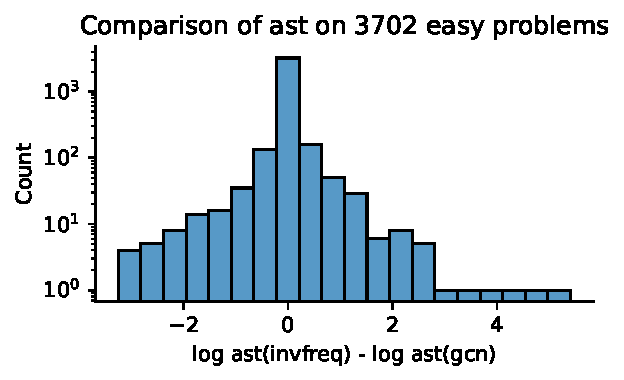
\includegraphics[scale=.5]{data/ast.pdf}
\end{exampleblock}}
\end{frame}
\begin{frame}{Question 2}
\begin{block}{Question}
What methods are considered to be applied for integration of the proving strategy and schedule optimization?
\end{block}
\begin{exampleblock}{Answer}
Combine \gls{smbo} with fast schedule optimization. Iteratively construct a portfolio:
\begin{enumerate}
\item Train a probabilistic \gls{epm}.
\item Estimate value of new strategies using the \gls{epm},
empirical runtimes of the portfolio, and
fast schedule optimization.
\item Empirically evaluate the best strategy.
\item Expand the portfolio if the new strategy improves it.
\end{enumerate}
\end{exampleblock}
\end{frame}
\begin{frame}{Question 0}
\begin{block}{Question 0}
Will these datasets be available for re-use by public?
\end{block}
\begin{exampleblock}{Comment}
The source code has been published.

I hope to publish the datasets when I consolidate the results for my dissertation thesis.
\end{exampleblock}
\end{frame}


\section{Technical details}

\begin{frame}
\frametitle{Notation overview}
\begin{center}
\begin{tabular}{ll}
$\pi(i)$ & index of the $i$-th symbol in precedence $\pi$ \\
$c$ & vector of symbol costs (output of the \acrshort{gcn}) \\
$c_i$ & cost of the $i$-th symbol \\
$C(\pi)$ & cost of symbol precedence $\pi$ \\
$\loss(P, \PrecBetter, \PrecWorse)$ & loss for training example $\Better{\PrecBetter}{\PrecWorse}{P}$ \\
\end{tabular}
\end{center}
\end{frame}

\begin{frame}
\frametitle{Prediction of symbol precedence $\pi$}
\begin{algorithmic} % enter the algorithmic environment
\REQUIRE Problem $P$
\ENSURE Symbol precedence $\pi$
\STATE $c \gets \mathrm{\acrshort{gcn}}(P)$
\COMMENT {Forward pass through the \acrshort{gcn} to obtain vector of symbol costs $c$}
\STATE $\pi \gets \argsort^- (c_1, \ldots, c_n)$
\COMMENT {Sort symbols by $c$ in non-increasing order to obtain precedence $\pi$}
\RETURN $\pi$
\end{algorithmic}
\end{frame}

\begin{frame}
\frametitle{\Acrfull{gcn}}

Initial embedding of node $d$:
$$
h_d^{(0)} = \textrm{(feature vector)} \oplus \textrm{(trainable vector)}
$$

Feature vector:
\begin{itemize}
\item Clause: role (axiom, assumption, negated conjecture)
\item Symbol: introduced in preprocessing, in conjecture
\end{itemize}

Propagation rule for layer $l$:
$$
h_d^{(l+1)} =
\sum_{r \in \mathcal{R}} \sigma \Parentheses*{\sum_{s \in \mathcal{N}_d^r} \frac{1}{\sqrt{\card{\mathcal{N}_s^r}} \sqrt{\card{\mathcal{N}_d^r}}} (W_r^{(l)} h_s^{(l)} + b_r^{(l)})}
$$

\end{frame}

\section{Training}

\begin{frame}
\frametitle{Precedence cost}
Reminder: $c_i$ is the cost of the $i$-th symbol.

\begin{block}{Cost of symbol precedence $\pi$ over signature of length $n$}
\begin{equation*}
C(\pi) = \frac{2}{n(n+1)} \sum_{i=1}^n i \cdot c_{\pi(i)}
\end{equation*}
\end{block}

\begin{lemma}[Precedence cost minimization]
The precedence cost $C$ is minimized by any precedence that sorts the symbols by their costs in non-increasing order:
$$
\argmin_{\rho \in \mathrm{Perm}(n)} C(\rho) = \argsort^- (c_1, \ldots, c_n)
$$
\end{lemma}

\end{frame}

\begin{frame}
\frametitle{Proof sketch: Precedence cost minimization}

$C(\pi) = \frac{2}{n(n+1)} \sum_{i=1}^n i \cdot c_{\pi(i)}$

\begin{lemma}[Precedence cost minimization]
$$
\argmin_{\rho \in \mathrm{Perm}(n)} C(\rho) = \argsort^- (c_1, \ldots, c_n)
$$
\end{lemma}

\newcommand{\StairsSorted}{

\begin{tikzpicture}[baseline=5pt]
\begin{axis}[ybar interval=1, axis lines=none, height=60pt, width=60pt]
\addplot[black] coordinates {(1,5) (2,4) (3,3) (4,2) (5,1) (6,0)};
\end{axis}
\end{tikzpicture}
}

\newcommand{\StairsUnsorted}{

\begin{tikzpicture}[baseline=5pt]
\begin{axis}[ybar interval=1, axis lines=none, height=60pt, width=60pt]
\addplot[black] coordinates {(1,5) (2,3) (3,4) (4,2) (5,1) (6,0)};
\end{axis}
\end{tikzpicture}
}

\begin{example}
$$
C\Parentheses*{\StairsSorted} < C\Parentheses*{\StairsUnsorted}
$$

Proof:
\begin{align*}
C\Parentheses*{\StairsUnsorted} - C\Parentheses*{\StairsSorted}
&\propto ((2 \cdot 3 + 3 \cdot 4) - (2 \cdot 4 + 3 \cdot 3)) \\
&= 18 - 17 = 1 > 0
\end{align*}
\end{example}

\end{frame}

\begin{frame}
\frametitle{Loss function}

\begin{exampleblock}{Training example $\Better{\PrecBetter}{\PrecWorse}{P}$}
Precedence $\PrecBetter$ is better than precedence $\PrecWorse$ for problem $P$.
\end{exampleblock}

Reminder: $C(\pi)$ is the predicted cost of precedence $\pi$.

\begin{block}{Loss on training example $\Better{\PrecBetter}{\PrecWorse}{P}$}
\begin{equation*}
\loss(P, \PrecBetter, \PrecWorse) = - \log \sigmoid (C(\PrecWorse) - C(\PrecBetter))
\end{equation*}

\centering
% https://pgf-tikz.github.io/pgf/pgfmanual.pdf : 94. Mathematical Expressions
\begin{tikzpicture}
\begin{axis}[
    domain=-12:12,
    xmin=-12,
    xmax=12,
    ymin=-1,
    ymax=11,
    samples=100,
    xlabel={$C(\PrecWorse) - C(\PrecBetter)$},
    ylabel={$\loss(P, \PrecBetter, \PrecWorse)$},
    scale only axis,
    width=0.5\textwidth,
    height=0.25\textwidth
]
%\addplot[gray] {0};
%\addplot[gray] {-x};
\addplot[] {-ln(\FuncSigmoid(x))};
\end{axis}
\end{tikzpicture}
\end{block}

\end{frame}

\begin{frame}
\frametitle{Concise representation of training examples}
\begin{block}{Cost of symbol precedence $\pi$ over signature of length $n$}
\begin{equation*}
C(\pi)
= \frac{2}{n(n+1)} \sum_{i=1}^n i \cdot c_{\pi(i)}
= \frac{2}{n(n+1)} \sum_{i=1}^n c_i \cdot \inv{\pi}(i)
\end{equation*}
\end{block}

\begin{block}{Loss of training example $\Better{\PrecBetter}{\PrecWorse}{P}$}
\begin{align*}
\loss(P, \PrecBetter, \PrecWorse)
&= - \log \sigmoid (C(\PrecWorse) - C(\PrecBetter)) \\
&= - \log \sigmoid \frac{2}{n(n+1)} \sum_{i=1}^n i (c_{\PrecWorse(i)} - c_{\PrecBetter(i)}) \\
&= - \log \sigmoid \frac{2}{n(n+1)} \sum_{i=1}^n c_i (\inv{\PrecWorse}(i) - \inv{\PrecBetter}(i))
\end{align*}
\end{block}

Concise representation of $\Better{\PrecBetter}{\PrecWorse}{P}$:
$\inv{\PrecWorse} - \inv{\PrecBetter}$
\end{frame}

\section{Impact of precedence on rewriting}

\begin{frame}
\frametitle{Precedence determines orientability of identities}
$$
f(x, a, y) \approx f(y, b, x)
$$

\begin{itemize}
\item If $a > f$ and $a > b$,
then $f(x, a, y) >_{lpo} f(y, b, x)$.
\item If $f > a$ and $f > b$,
then $f(x, a, y)$ and $f(y, b, x)$ are $>_{lpo}$-incomparable.
\end{itemize}
\end{frame}

\begin{frame}
\frametitle{Precedence determines termination of completion}
Set of identities:
\begin{align*}
x + 0 &\approx x \\
x + s(y) &\approx s(x + y)
\end{align*}

\begin{itemize}
\item LPO($+ > s$):
Completion orients from left to right and terminates.
\item LPO($s > +$):
% See TRaAT, Example 7.1.3
Completion diverges:
\begin{align*}
x + 0 &\to x\\
x + s(0) &\to s(x)\\
x + s(s(0)) &\to s(s(x))\\
&\vdots\\
x + s^n(0) &\to s^n(x)\\
&\vdots
\end{align*}
\end{itemize}
\end{frame}

\begin{frame}
\frametitle{Precedence may inflate the search space}
\begin{enumerate}
\item $>_{+s}$ = LPO($* > + > s$)
\item $>_{s+}$ = LPO($s > + > *$)
\end{enumerate}
\begin{align*}
x + 0 &\to x \\
x + s(y) &\approx s(x + y) \tag{$\to_{+s}$, $\leftarrow_{s+}$}\\
x * 0 &\to 0\\
x * s(y) &\to x + (x * y)
\end{align*}
\begin{enumerate}
\item With $>_{+s}$, the initial set is complete.
\item With $>_{s+}$, completion yields a large number of new rules:
\begin{align*}
x + s^n(0) &\to s^n(x) \tag{$\forall n \in \nat$}\\
x + (x * (x' + y')) &\approx x * (x' + s(y')) \tag{unorientable}
\end{align*}
\end{enumerate}
\end{frame}

\end{document}
